\subsection{Descripci\'on del problema}

En este punto se nos pide resolver el problema de ubicar centrales de gas de manera estrat\'egica entre los pueblos de una cierta regi\'on.\\

Dados $n$ pueblos con sus respectivas coordenadas en el plano y $k$ centrales de gas, la idea es ubicar las centrales en algunos de los pueblos. Luego es posible construir tuber\'ias entre pueblos; una tuber\'ia que va de un pueblo con central a uno sin no s\'olo transporta el gas a este \'ultimo sino que adem\'as lo convierte en potencial proveedor. Es decir que se da una especie de transitividad entre pueblos: si un pueblo $a$ con central de gas se conecta a otro pueblo $b$ y a su vez $b$ se conecta con $c$ entonces $c$ tambi\'en recibe gas.\\

El \'unico problema que presentan las tuber\'ias es que, a mayor longitud aumenta la posibilidad de rotura de las mismas. Evidentemente \'este es un factor que se quiere evitar, por lo cual se nos pide que, al elegir los pueblos donde instalar las centrales y y las conecciones entre pueblos minimicemos el tama\~o de la tuber\'ia m\'as larga.\\

Veamos algunos ejemplos, la siguiente es una situacion trivial en la que tenemos la misma cantidad de pueblos que de centrales:

\begin{figure}[h]
\begin{center}
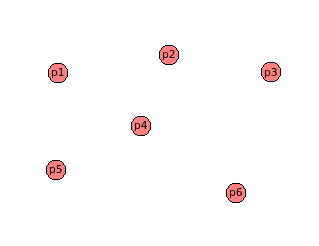
\includegraphics[scale=0.7]{./img/ej2_explicacion1.png}
\caption{Caso trivial}
\end{center}
\end{figure}

Los circulos colorados indican donde fueron instaladas las centrales, en este caso no hay ninguna tuber\'ia.\\

Veamos el siguiente caso mas complejo: 

\begin{figure}[h]
\begin{center}
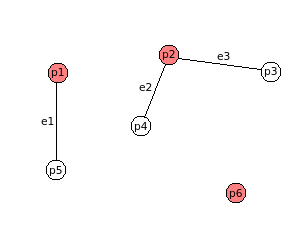
\includegraphics[scale=0.7]{./img/ej2_explicacion2.png}
\caption{Caso con K = 3 y N = 6}
\end{center}
\end{figure}

Como dato, sabemos que $e_2 < e_3 < e_1$ con lo cual nuestro largo m\'aximo de tuber\'ia es $e_1$

\subsection{Resoluci\'on}

Para resolver el problema dado decidimos modelarlo con grafos de tal forma que los nodos representen los pueblos, y las aristas (con pesos) las posibles conexiones entre pueblos. Estos pesos estan basados en las distancias entre cada par de pueblos. \\

Como se nos pide minimizar el riesgo de rotura de las tuber\'ias a instalar, lo ideal ser\'ia lograr un esquema de conexi\'ones tal que el largo de la tuber\'ia mas larga sea m\'inimo. Como veremos mas adelante, la ubicaci\'on de las centrales de gas no es de gran importancia ya que la transimisi\'on del servicio de gas se da por transitividad entre pueblos conectados (mientras alguno tenga una central). Lo importante es tener grupos de pueblos conectados a una misma central de tal manera que estas tuberias sean de tama\~no m\'inimo, sin importar la cantidad de tuberias usadas. \\

Como primer paso decidimos guardar en una estructura de datos de cola de prioridad (implementada en un Heap) todos los pares de distancias entre pueblos, de menor a mayor. Esto nos permite saber que el primer elemento del Heap posee al par de pueblos mas cercanos de todo el mapa, y cada vez que pidamos el proximo tendremos pares de pueblos de distancia minima, pero mayor o igual que el anterior. Cabe recordar que la distancia entre el puebo A posicionado en la coordenada $(x_0,y_0)$ y el pueblo B posicionado en la coordenada $(x_1,y_1)$ es igual a $\sqrt{(x_1-x_0)^2+(y_1-y_0)^2}$ \\

Una vez obtenida esta informaci\'on, nuestro mapa empieza con 0 conexiones entre pueblos y N pueblos, resultando un grafo de N componentes conexas. La clave esta en conseguir K (cantidad de centrales de gas) componentes conexas con largo de tuber\'ias m\'inima. Notar que puede ocurrir que K sea mayor o igual a N, con lo que el problema se vuelve trivial. \\

Realizamos un ciclo que, a cada paso, verifica si no logramos tener las K componentes conexas. Caso contrario agregamos una nueva conexion entre el pr\'oximo par de pueblos mas cercano que no compartan la misma componente conexa, logrando asi decrementar la cantidad de componentes conexas cada vez que se satisface esta condici\'on. Finalmente el ciclo terminar\'a al lograr las K componentes conexas y el \'ultimo paso es ubicar las K centrales en alg\'un pueblo de cada una de estas componentes.\\

Con esto logramos repartir gas a todos los pueblos sin generar conexiones innecesarias.

\subsection{Demostraci\'on de la resoluci\'on}

\subsection{Complejidad del algoritmo}

Veamos la complejidad del algoritmo propuesto utilizando un pseudoc\'odigo que facilite el an\'alisis.\\

Analicemos primero el constructor de regi\'on. S\'olo vamos a ver la parte en que se crea la lista de pares de ciudades ordenada de menor a mayor seg\'un la distancia entre ellas ya que el resto del constructor solamente hace asignaciones a variables (ver en la secci\'on siguiente).
\begin{itemize}
\item poner i $\leftarrow$ 1
\item para cada pueblo en pueblos  \/// O(n) 
\begin{itemize}
	\item poner j $\leftarrow$ 1
	\item para cada pueblo2 en pueblos \/// O(n)
	\begin{itemize}
		\item si i > j entonces poner pueblos $\leftarrow$ (pueblo, pueblo2) y poner porDistancia $\leftarrow$ (pueblos, distancia(pueblo, pueblo2))
		\item poner j $\leftarrow$ j + 1
	\end{itemize}
	\item poner i $\leftarrow$ i + 1
\end{itemize}
\item ordenar porDistancia \/// O(n*log(n)) 
\end{itemize}

Por el for anidado que tenemos, que nos lleva a recorrer dos veces la lista de pueblos, obtenemos una complejidad de $O(n^2)$

\subsection{C\'odigo fuente}

\lstset{language=C++,
                basicstyle=\ttfamily\footnotesize,
                keywordstyle=\color{blue}\ttfamily,
                stringstyle=\color{red}\ttfamily,
                commentstyle=\color{green}\ttfamily,
                morecomment=[l][\color{magenta}]{\#},
                breaklines=true
}
\begin{lstlisting}


/* Constructor de region
 * notar: crea la lista de pares de ciudades ordenada por distancia de menor a mayor
**/
Region::Region(list<Pueblo*> * lista_pueblos, int centralitas){
	
	_centralitas = centralitas;
	_centrales_instaladas = 0;
	_tuberias_instaladas = 0;
	_pueblos = lista_pueblos;
	_pueblos_conectados_ady = new vector< vector<bool> >(_pueblos->size()+1, vector<bool>(_pueblos->size()+1, false) );
	_cant_grupos_pueblos = _pueblos->size();
	_pueblos_por_distancia = new list< pair<pair<Pueblo*,Pueblo*>, double> >();
	
	int i = 1;
	for(list<Pueblo*>::iterator p = _pueblos->begin(); p != _pueblos->end(); p++){
		
		int j = 1;
		for(list<Pueblo*>::iterator p2 = _pueblos->begin(); p2 != _pueblos->end(); p2++){
			
			// Para evitar guardar la distancia simetrica
			if(i > j){
				pair<Pueblo*, Pueblo*> pueblos = pair<Pueblo*, Pueblo*>(*p,*p2);
				pair< pair<Pueblo*, Pueblo*>, double> data = pair<pair<Pueblo*, Pueblo*>, double>(pueblos,(**(p)).distancia(**p2));
				_pueblos_por_distancia->push_back(data);
			}
			
			j++;
			
		}
		i++;
	}
	
	// Dejo ordenada la lista de distancias
	_pueblos_por_distancia->sort(pairCompare);
	
}

void Region::resolver(){
	
	list<pair<pair<Pueblo*,Pueblo*>, double> >::iterator pueblos_distancia_it = _pueblos_por_distancia->begin();
	

	// Mientras no logre k componentes conexas para alimentar a todos los pueblos sigo conectando
	while(_centralitas < _cant_grupos_pueblos){
		
		// Conecto los pueblos mas cercanos disponibles
		pair< pair<Pueblo*, Pueblo*>, double> data = *pueblos_distancia_it;
		
		Pueblo * p1 = data.first.first;
		Pueblo * p2 = data.first.second;
		
		// Si estan en componentenes conexas distintas las uno
		if(p1->getIdGrupoPueblo() != p2->getIdGrupoPueblo()){
		
			(*_pueblos_conectados_ady)[p1->getId()][p2->getId()] = true;
			(*_pueblos_conectados_ady)[p2->getId()][p1->getId()] = true;
			
			// Junto las clases de equivalencia
			int id_grupo_viejo = p2->getIdGrupoPueblo();
			
			for(list<Pueblo*>::iterator p = _pueblos->begin(); p != _pueblos->end(); p++){
				if((**p).getIdGrupoPueblo() == id_grupo_viejo){
					(**p).setIdGrupoPueblo(p1->getIdGrupoPueblo());
				}
			}
			
			_cant_grupos_pueblos--; // La cantidad de componentes conexas siempre disminuye ya que conecto pueblos sueltos a cada paso
			_tuberias_instaladas++;
		
		}
		
		pueblos_distancia_it++;
		
	}

	// Dicc para saber en que componentes conexas ya instale una central
	map<int, bool> * grupos_instalados = new map<int, bool>();
	
	for(list<Pueblo*>::iterator p = _pueblos->begin(); p != _pueblos->end(); p++){
		
		if(grupos_instalados->find((*p)->getIdGrupoPueblo()) == grupos_instalados->end()){
			(*p)->instalarCentral();
			(*grupos_instalados)[(*p)->getIdGrupoPueblo()] = true;
			_centrales_instaladas++;
		}
		
	}
	
	delete grupos_instalados;	
}

\end{lstlisting}

\subsection{Casos de prueba}

\subsection{Performance}
